\documentclass[class=report, crop=false]{standalone}
\usepackage{mathtools}
\DeclarePairedDelimiter\ceil{\lceil}{\rceil}
\usepackage[shortlabels]{enumitem}
% make sure to keep these two lines the very last in the preamble
% if you want to add packages add them before not after these two lines
\usepackage[subpreambles=true]{standalone}
\usepackage{import}
\begin{document}
    Après une étude ciblée des travaux existants sur le problème du Bin Packing, nous avons abouti à une synthèse des méthodes de résolution les plus connues --dans chacune des trois catégories: méthodes exactes, et méthodes approchées: heuristiques et métaheuristiques-- que nous allons exposer dans ce qui suit. 
    \section{Méthodes Exactes}
    Les méthodes exactes permettent d’avoir des solutions optimales, cependant le temps de calcul peut être très long pour certaines instances du problème. Il n’existe pas un grand nombre de méthodes exactes pour résoudre le problème du Bin Packing , nous allons présenter dans ce qui suit la méthode  MTP ( basée sur le Branch and Bound) et une méthode de programmation dynamique DP-flow.
    \subsection{Branche and Bound}
    Cette méthode a été  utilisée pour la première fois dans les années \\ cinquante pour résoudre qui a été  modélisé par un programme linéaire en nombres entiers.
Afin de rendre le processus de résolution plus rapide, cet algorithme utilise une borne inférieure. Plusieurs techniques ont été proposés pour obtenir cette dernière.
    \paragraph{Borne inférieure évidente:} Soient \(C\) la capacité des boîtes utilisés,\\
     \(A\) l’ensemble des articles \(a_i\) de volumes \(v_i\) de l’instance \(I\).
        \[BI(I)=\frac{\displaystyle\sum_{i=1}^{n} v_i}{C}\]
    \paragraph{Borne de Martello and Toth \(L_2\):}  
    Soit \(\alpha\) un entier tels que :
    \[0 \le \alpha \le C/2\]
    On definie des classes d'articles suivantes: 
    \[C_1 = \{a_i, \quad C-\alpha < v_i\} \]
    \[C_2 = \{a_i, \quad C/2 < v_i \le C-\alpha\} \]
    \[C_3 = \{a_i, \quad \alpha < v_i \le C/2\} \]
    \(BI(I)\)  est donnée par la formule suivante:
    \[BI(I)=max\{L(\alpha),\quad 0 \le \alpha \le C/2\}\]
    Avec
    \[L(\alpha)=|C_1|+|C_2|+max(0, \ceil*{\frac{\sum_{j \in C_3}^{} v_j - (|C_2|*C - \sum_{j \in C_2}^{} v_j) }{C}})\]
    cette borne est calculé en un temps \(o(nlogn)\).
    \paragraph{Borne inférieure  \(L_3\):}
    Une autre technique a été utilisé dans l’algorithme de résolution MTP pour déterminer une borne inférieure.
    Soient \(n_1\) le nombre de boîtes obtenus après la première application de la technique de réduction MTP qui consiste à réduire l’instance du problème en rangeant l’article le plus petit, soit \(Ir^1\) l’instance résiduelle de l’instance \(I\) après cette première application ie l’ensemble des articles restants après l’opération de réduction
    \[L^\prime_1=n_1+L_2(Ir^1) \ge L_2(I)\]
    On refait ce processus jusqu'à ce que l’instance résiduelle soit vide (i.e.: tous les articles ont été rangés). A l’itération \(k\), on obtiendra :
    \[L^\prime_K= \displaystyle\sum_{i=1}^{k} n_i + L_2(Ir^k)\] 
    La borne inférieure \(L_3\) est obtenue en appliquant la formule suivante , par la suite :
    \[L_3=max \{L^\prime_1, L^\prime_2,\cdots,L^\prime_{kmax}\}\]
    \textbf{Un des algorithmes proposés pour cette méthode est l’algorithme MTP:} 
    \subsubsection*{L’algorithme MTP (Martello and Toth Procédure):}
    Le meilleur algorithme existant pour trouver la solution optimale du problème Bin Packing est celui proposée par  \emph{Martello et Toth (Martello \& Toth 1990a; 1990b)} [1] le principe est le suivant :  
Les articles sont initialement triés selon des poids décroissants. À chaque nœud de décision, le premier élément libre est attribué, à son tour, aux boîtes existantes qui peuvent le contenir (on parcourt les boîtes par ordre de création) et à une nouvelle boîte. 
À chaque nœud de l'arbre de recherche 
\begin{enumerate}[a.]
    \item Une borne inférieure \(L_3\) de la solution restante est calculée et utilisée pour élaguer le nœud de l'espace de recherche et réduire le problème actuel.
        \begin{itemize}
            \item Si la borne inférieure du nœud actuel est supérieure \\
            à la borne inférieure du problème d’origine (nœud racine), le nœud est supprimé. Sinon (b)
        \end{itemize}
    \item Des algorithmes approximatifs FFD, BFD et WFD (qu’on présentera dans la partie Méthodes approximatives) sont appliqués au problème actuel, et chacune des solutions approximatives obtenues est comparée à la borne inférieure \(L_3\).
        \begin{itemize}
            \item Si le nombre de boîtes utilisées par l'une des solutions approximatives est égal à la borne inférieure du nœud actuel, aucune autre recherche n'est effectuée sous ce nœud. 
            \item Si le nombre de boîtes utilisées dans une solution approximative est égal à la borne inférieure \(L_3\) du problème d'origine (nœud racine), l'algorithme se termine, renvoyant cette solution comme optimale.
        \end{itemize}
\end{enumerate}
De plus, La principale source d'efficacité de l'algorithme de Martello et Toth est une méthode pour réduire la taille des sous-problèmes restants, appelée \textbf{critère de dominance}.
    \subsection{Programmation Dynamique}
    La programmation dynamique est une méthode algorithmique pour résoudre des problèmes d'optimisation. Le concept a été introduit au début des années 1950 par Richard Bellman. Elle consiste à résoudre un problème en le décomposant en sous-problèmes, puis à résoudre les sous-problèmes, des plus petits aux plus grands en stockant les résultats intermédiaires.
    Elle s'appuie sur \emph{le principe d'optimalité de Bellman}: une solution optimale d'un problème s'obtient en combinant des solutions optimales à des sous-problèmes. 
    Un modèle pseudo-polynomial simple, pour résoudre le problème bin-packing, est obtenu en associant des variables aux décisions prises dans une table de programmation dynamique (DP) classique.
        \subsubsection*{DP-flow:}
        Dans le modèle BPP proposé par \emph{Cambazard et O’Sullivan} [2], connu sous\\
        le nom de DP-flow, les états DP sont représentés par un graphique dans \\
        lequel un chemin qui commence à partir d'un nœud initial et se termine à \\ 
        un nœud terminal représente un remplissage possible d'une boîte. Notons \\
        \((j, d) (j = 0, \cdots, n \, et \, d = 0, \cdots, c)\) un état DP où les articles de \(0\) à \(j\) ont déjà \\
        été étudié (les décisions de placer les articles de \(0\) à \(j\) dans la boîte ou non\\
        ont déjà été reprises ) et entraînent un remplissage partiel de la boîte de \(d\) \\
        unités. Notons également par \(((j, d), (j + 1, e))\) un arc reliant les états \((j, d)\) \\
        et \((j + 1, e)\). Un tel arc exprime la décision d'emballer ou non l'article \(j + 1\) à partir de l'état actuel \((j, d)\): l'état atteint par l'arc est \((j + 1, d + w_j + 1)\) si l'article \(j + 1\) est emballé, et \((j + 1, d)\) sinon.
        Soit \(A\) l'ensemble de tous les arcs. Comme un remplissage réalisable d’une boîte est représenté par un chemin qui commence à partir du nœud \((0, 0)\) et se termine au nœud \((n + 1, c)\), le BPP consiste à sélectionner le nombre minimum des chemins qui contiennent tous les éléments. \\
        Pour cette instance BPP, une solution optimale est produite par les deux chemins mis en évidence dans la figure ci-dessous, à savoir \\\([(0,0), (1,4), (2,4), (3,7), (4,7), (5,9), (6,9), (7,9)]\) \\
        et \([(0,0), (1,0), (2,4), (3,4), (4,7), (5,7), (6,9), (7,9)]\).
        \begin{figure}[h!]
            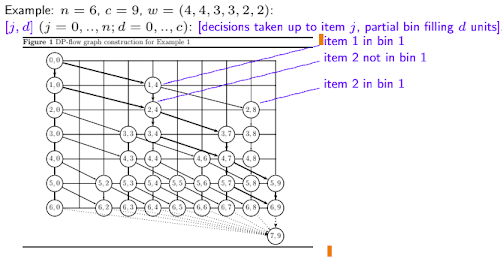
\includegraphics[width=13.5cm]{../figures/DP-flow.png}
        \end{figure}

        \section{Heuristiques}
        Les méthodes approchées  sont classées en plusieurs catégories:
        \subsection{Algorithmes ON-LINE:}
        Ces algorithmes considèrent l’hypothèse que les articles arrivent un à la fois en un ordre connu, chaque article doit être rangé avant de passer à l’article suivant.
        \subsubsection{Next Fit (NF):} Lors du rangement de l’article a, NF vérifie s'il tient dans la même boîte que le dernier article (Soit la boîte du dernier article rangé Bj). Si c’est le cas, il place l’article dans la boîte Bj, laissant cette boîte ouverte. Sinon, il ferme la boîte Bj et place l’article a dans une nouvelle boîte Bj+1, qui devient maintenant la boîte ouverte. 
        \\ \textbf{Remarque:} \\
        Il existe des variants pour cet algorithme, permettant d’améliorer ses performances : 
        \begin{itemize}
            \item \textbf{Next-KFIT (NFk): } autorise k boîte ouvertes à la fois, c’est à dire qu’il vérifie dans les K boîtes ouvertes s’il y a assez d’espace pour ranger l’article a, sinon il ouvre une nouvelle boîte. Si K=1 on retombe sur l’algorithme NF.
        \end{itemize}
        \subsubsection{First Fit (FF): } Lors du rangement de l’article a, NF vérifie s'il tient dans la même boîte que le dernier article (Soit la boîte du dernier article rangé Bj). Si c’est le cas, il place l’article dans la boîte Bj, laissant cette boîte ouverte. Sinon, il ferme la boîte Bj et place l’article a dans une nouvelle boîte Bj+1, qui devient maintenant la boîte ouverte. 
        \subsubsection{Best Fit (BF):} L’article a est rangé dans une des boîtes ouvertes de sorte que le plus petit espace vide soit laissé. Si l’article ne tient dans aucune boîte existante, il sera placé dans une nouvelle boîte. 
        \\ \textbf{Remarque:} \\
        Il existe des variants pour cet algorithme, permettant d’améliorer ses performances : 
        \renewcommand{\labelitemi}{$\circ$}  
        \begin{itemize}
            \item \textbf{K-Bounded Best Fit (BBFk): } utilise le même principe que Best Fit, sauf qu’il restreint le nombre de boîtes ouvertes à k boîtes. ie : l’article a est rangé dans une des k-boîtes ouvertes de sorte que le plus petit espace vite soit laissé. 
        \end{itemize}
        \subsubsection{Worst Fit (WF): }L’article a est rangé dans la boîte avec le plus grand espace vide, si cette dernière ne peut pas contenir l’article, il sera placé dans une nouvelle boîte.
        \\ \textbf{Remarque:} \\
        Il existe des variants pour cet algorithme, permettant d’améliorer ses performances : 
        \renewcommand{\labelitemi}{$\circ$}  
        \begin{itemize}
            \item \textbf{Almost Worst Fit (AWF): }l’article a est rangé dans la 2ème boîte la plus vide, jusqu’à ce qu’il reste qu’une seule boîte qui peut contenir l’article. Dans ce cas il est placé dans cette boîte. Si l’article ne tient dans aucune boîte existante, il sera placé dans une nouvelle boîte.
        \end{itemize}
        \subsubsection{Harmonic K (Hk): } Cet algorithme est basé sur une partition de l'intervalle \([0,1]\) en \(K\) sous-intervalles \(I_k\), où  \(I_k=]\frac{1}{K + 1};\frac{1}{K}]\), à chacun de ces sous-intervalles correspond une seule boîte ouverte, et seuls les articles appartenant à ce sous-intervalle (i.e.: \(v_i / C \in I_k\) avec \(v_i\) le volume d'un article) sont regroupés dans cette boîte. Si un nouvel article arrive et ne rentre pas dans sa boîte ouverte correspondante, la boîte est fermée et une nouvelle boîte est ouverte.
        \\ \textbf{Remarque:} \\
        Il existe des variants pour cet algorithme, permettant d’améliorer ses performances : 
        \renewcommand{\labelitemi}{$\circ$}  
        \begin{itemize}
            \item \textbf{Simplified HarmonicK (SHk): } se base sur une structure d’intervalle qui est plus compliquée.
        \end{itemize}
        \subsubsection{Autres algorithmes: }
        \renewcommand{\labelitemi}{$\circ$}  
        \begin{itemize}
            \item \textbf{ABFk: } utilise le principe de rangement du Best Fit avec le principe de fermeture des boîtes du First Fit.
            \item \textbf{AFBk: } utilise le principe de rangement du First Fit avec le principe de fermeture des boîtes du Best Fit.
        \end{itemize}
        \textbf{Remarque: } \\
        Dans le cas où \(K=1\), ces algorithmes sont équivalent à l’algorithme Next Fit. 
        \subsection{Algorithmes OFF-LINE: }
        Dans ce type d’algorithmes on a accès à tous les articles avant de commencer le rangement dans les boîtes. 
        \emph{Quelques algorithmes off-line:}
        \subsubsection{First Fit Decreasing (FFD) : }
        Ordonner les articles par ordre décroissant des poids, ensuite appliquer l’algorithme First Fit.
        \subsubsection{Best Fit Decreasing (BFD) :}
        Ordonner les articles par ordre décroissant des poids, ensuite appliquer l’algorithme Best Fit
        \subsection{Algorithmes SEMI-ONLINE :}
        Les algorithmes dits semi-en ligne (SOL) se situent entre les online et les offline. Ils relâchent la prescription online de manière à permettre quelques opérations supplémentaires où l'algorithme a un peu de connaissance de l'avenir, au moins une des opérations suivantes est autorisée: comme reconditionner un nombre fini d'articles déjà emballés, prétraiter les articles en les commandant en fonction des tailles ou en tamponnant certains articles avant de les emballer. 
        \emph{Quelques algorithmes semi-online:}
        \subsubsection{MMP (Mostly Myopic Helps) : Fully Dynamic Algorithm}
        Dans cet algorithme [3], en partant de l’hypothèse que l'emballage peut être réarrangé arbitrairement pour accueillir les articles arrivant et partant, on suppose :
        \renewcommand{\labelitemi}{$\circ$}  
        \begin{itemize}
            \item l’emballage d’un article se fait en une abstraction totale des articles déjà emballés d’une taille plus petite(c’est à dire, on suppose que leurs places dans les boîtes sont vides, où le nouvel article pourra être affecté dans cet espace, et ces articles de petites tailles pourront être réarrangés).
            \item Regroupement des articles plus petits dans des lots(un groupe d'articles plus petit que \(\epsilon\) peut être déplacé comme un seul article).
            \item Le nombre d'articles uniques ou de lots de très petits articles qui doivent être réarrangés est délimité par une constante.
        \end{itemize}
        Cet algorithme nécessite du temps \(\Theta(\log n)\) par opération (c'est-à-dire pour une insertion ou une suppression d'un article). Il est presque aussi bon que celui des meilleurs algorithmes offlines pratiques.
        \subsubsection{Harmonic Fit avec (4 ou 6) partitions: }
        Le HF avec 4 partitions [4], en utilisant une structure de données appropriée, permet de traiter de grandes collections de petits articles en :
        \renewcommand{\labelitemi}{$\circ$}  
        \begin{itemize}
            \item les groupant et les déplaçant tous à la fois en temps constant
            \item les classifiant en 4 types par taille
            \item ne permettant au plus que les déplacements de 3 lots d’articles ou d'un seul article lorsqu'un nouvel article doit être attribué
        \end{itemize}
        Le HF avec 6 partitions [4] utilise:
        \renewcommand{\labelitemi}{$\circ$}  
        \begin{itemize}
            \item six types d'articles classés par taille
            \item au plus 7 mouvements de lots/ article par nouvel article
        \end{itemize}
        \subsection{Algorithmes d’Espace Borné (Bounded Space):}
        les algorithmes décident où un élément doit être emballé sur la base du contenu actuel d'un nombre fini k de bacs, où k est un paramètre de l'algorithme. Notez que FF et BF ne sont pas des algorithmes d'espace bornés, mais NF l'est, avec \(k = 1\).
        \section{Métaheuristiques}
        \subsection{La recherche tabou: }
        Une méthode de résolution a été proposée par Fernandes Muritiba Et al.[5] ,qui prend en entrée une population initiale obtenue par une heuristique et applique un opérateur de croisement sur ces solutions .Chaque solution obtenue est améliorée par la suite en utilisant une recherche tabou, qui consiste à  se déplacer dans un espace de recherche contenant des solutions réalisables  partielles où certains articles ne sont pas affectés à des boîtes. L’amélioration consiste de passer d’une solution partielle de valeur K à une solution complète de la même valeur. La fonction objective utilisée est basée sur la somme pondérée des tailles des articles.
Pour la diversification de l’espace de recherche, On utilise une procédure basée sur un opérateur de croisement.
        \subsection{L’algorithme ILWOA (Improved Lévy WOA): }
        L’algorithme WOA (Whale Optimization Algorithm) [6] est basé sur une méthode inspirée de la nature plus exactement d’une stratégie d’alimentation des baleines à bosse, où la recherche des proies représente l’exploration de l’espace de recherche et la libération des bulles représente l’exploitation.
Une amélioration de cet algorithme a été proposée par Abdel-Basset, M., Manogaran, G., Abdel-Fatah, L. et al [7].Il s’agit de l’utilisation de fonctions logistiques et d’autres méthodes probabilistes pour assurer une convergence plus rapide
        \subsection{L’algorithme FFA (FireFly Algorithm): }
        L'algorithme FireFly (FFA) [8] est une métaheuristique génétique, inspirée par le comportement clignotant des lucioles. Le but principal du flash d'une luciole est d'agir comme un système de signal pour attirer d'autres lucioles. Il y a trois règles. La première règle, chaque luciole attire tous les autres lucioles avec des flashs plus faibles. Deuxièmement, l'attractivité est proportionnelle à leur luminosité qui est inversement proportionnelle à leurs distances. Pour deux lucioles clignotantes, la moins brillante se déplacera vers la plus brillante. L'attractivité est proportionnelle à la luminosité et ils diminuent tous les deux à mesure que leur distance augmente. S'il n'y en a pas plus brillant qu'une luciole particulière, il se déplacera de façon aléatoire. Enfin, aucune luciole ne peut attirer la luciole la plus brillante, cette dernière se déplace d’une façon aléatoire. Le FFA est construit par analogie, en appliquant ces trois règles sur une population de solutions initiale pour la faire évoluer en une population contenant la solution approchée.
\end{document}